\documentclass[12pt]{article}
\usepackage[left=0.9in, right=0.9in, top=0.7in, bottom=0.7in]{geometry}
\usepackage{tikz}
\usepackage{setspace}
\usepackage{hyperref}
\usepackage{amsfonts, amssymb, amsmath} 
\usepackage{titlesec}
\usepackage{pgfplots}
\pgfplotsset{compat=newest}
\usepackage{graphicx}
\usepackage{wrapfig}
\usepackage{caption}
\usepackage{enumitem}
\usetikzlibrary{shadows.blur}
\usepackage{graphicx}
\usepackage{lmodern}
\setlength{\parskip}{0pt}
\setlength{\parindent}{0pt}

\title{\textcolor{purple}{\Huge\textbf{Matematikai statisztika}}}

\renewcommand{\contentsname}{Tartalom}
\newcommand{\R}{\mathbb{R}}
\newcommand{\N}{\mathbb{N}}
\newcommand{\E}{\exists}
\newcommand{\mm}{\mathbf{m}}
\newcommand{\MM}{\mathbf{M}}
\newcommand{\K}{\mathbb{K}}
\newcommand{\D}{\mathcal{D}_f}

\definecolor{modernyellow}{HTML}{F4E4BC}
\definecolor{moderngreen}{HTML}{BDDCBD}

\tikzset
{
	definition/.style={
		draw,
		fill=white,
		line width=1pt,
		rounded corners,
		drop shadow={shadow blur steps=5,shadow xshift=1ex,shadow yshift=-1ex},
		text width=0.9\textwidth,
		inner sep=10pt
	},
	theorem/.style={
		draw,
		fill=white,
		line width=1pt,
		rounded corners,
		drop shadow={shadow blur steps=5,shadow xshift=1ex,shadow yshift=-1ex},
		text width=0.9\textwidth,
		inner sep=10pt
	},
	proof/.style={
		fill=white,
		rectangle,
		drop shadow={shadow blur steps=5,shadow xshift=1ex,shadow yshift=-1ex, gray},
		text width=0.9\textwidth,
		inner sep=6pt,
	},
	proof1/.style={
		fill=white,
		rectangle,
		drop shadow={shadow blur steps=5,shadow xshift=1ex,shadow yshift=0, gray},
		text width=0.9\textwidth,
		inner sep=6pt,
	}
}

\begin{document}
    \maketitle
    \tableofcontents

    \newpage
    \section{Előadás}
    \subsection{A statisztika fogalma és ágai}
    \textbf{Statisztika}: a valóság tömör, számszerű jellemzésére szolgáló tudományos módszertan, illetve gyakorlati tevékenység.
    Ágai:
    \begin{enumerate}
        \item \textbf{Leíró statisztika}: magába foglalja az információk összegyűjtését, összegzését, ábrázolását, tömör, számszerű jellemzését szolgáló módszereket
        \item \textbf{Matematikai statisztika}: matematikai tudomány, adatok feldolgozásáról, érteémezéséről és felhasználásáról szóló tudományos módszertan
    \end{enumerate}

    \subsection{Leíró statisztika alapfogalmak}
    \textbf{Statisztikai egység}: a statisztikai vizsgálat tárgyát képező egyed.\\
    \textbf{Statisztikai sokaság}: a megfigyelés tárgyát képező egyedek összessége, halmaza.\\
    \textbf{Statisztikai adat}: valamely sokaság elemeinek száma vagy a sokaság valamilyen másféle számszerű jellemzője, mérési eredmény.\\
    \textbf{Statisztikai ismérv}: a sokaság egyedeit jellemző tulajdonság.\\
    \textbf{Ismérvváltozatok}: az ismérvek lehetséges kimenetelei.\\
    \textbf{Minta}: a sokaság véges számosságú részhalmaza.\\
    \textbf{Statisztikai következtetés}:a valóságban a teljes sokaságot nem tudjuk vagy akarjuk megfigyelni, ezért csak az egyedek egy szűkebb csoportját figyeljük meg. A viszonylag kisszámú egyedre vonatkozó információk alapján szeretnénk a teljes sokaság egészére, egyes jellemzőire, tulajdonságaira érvényes következtetéseket kimondani.\\

    Példa:
    \begin{table}[ht]
        \centering
        \begin{tabular}{|l|l|}
            \hline
            Sokaság & most a teremben lévő homo sapiensek \\ \hline
            Statisztikai egység & a teremben lévő oktató \\ \hline
            Adat & a legmagasabb hallgató testtömegindexe \\ \hline
            Ismérv & nem \\ \hline
            Ismérvváltozatok & férfi, nő \\ \hline
            Minta & 5 véleténül választott hallgató \\ \hline
        \end{tabular}
    \end{table}
    
    \subsection{Csoportosítások, adatok fajtái}
    \textbf{Sokaságok csoportosítása}:
    \begin{enumerate}
        \item A sokaság egységeinek megkülönböztethetősége szerint:
        \begin{itemize}
            \item diszkrét: a sokaság egységei elkülönülnek egymástól
            \item folytonos: a sokaság egységeit nem tudjuk természetes módon elkülöníteni
        \end{itemize}
        \item A sokaság időpontra vagy időtartamra értelmezhető-e:
        \begin{itemize}
            \item álló: csak egy adott időpontra értelmezhető
            \item mozgó: csak egy adott időtartamra értelmezhető
        \end{itemize}
        \item A sokaság számossága szerint:
        \begin{itemize}
            \item véges
            \item végtelen
        \end{itemize}
    \end{enumerate}

    \textbf{A statisztikai adatok fajtái}:
    \begin{enumerate}
        \item alapadatok: közvetlenül a sokaságból származnak
        \item leszármaztatott adatok: alapadatokból műveletek eredményeként adódnak
    \end{enumerate}

    \textbf{Az ismérvek típusai}:
    \begin{enumerate}
        \item minőségi: az egyedek számszerűen nem mérhető tulajdonsága
        \item mennyiségi: az egyedek számszerűen mérhető tulajdonsága (diszkrét, folytonos)
        \item időbeli: az egységek időbeli elhelyezésére szolgáló rendezőelvek
        \item területi: az egységek térbeli elhelyezésére szolgáló rendezőelvek
        \item közös: tulajdonságok, amik szerint a sokaság egyedei egyformák
        \item megkülönböztető: azok a tulajdonságok, amik szerint a sokaság egyedei különböznek egymástól
    \end{enumerate}

    \textbf{Mérési skálák}
    \begin{enumerate}
        \item nominális: kódszámok a sokaság egyedeinek azonosítására, pl. utasok neme
        \item ordinális: valamely tulajdonság alapján való sorbarendezés, pl. az utasosztályok
        \item intervallumskála: a skálaértékek különbségei is valós információt adnak a sokaság egyedeiről. A skálán a nullpont meghatározása önkényes. Ilyen skálákhoz mértékegység is tartozik. pl. hőmérséklet
        \item  a skálának van valódi nullpontja is. Minden matematikai művelet elvégezhető ezekkel a számokkal. pl. kor, jegy ára
    \end{enumerate}

    \textbf{Statisztikai sor}: a sokaság egyes jellemzőinek felsorolása. Az ismérvek fajtája szerint beszélhetünk minőségi, mennyiségi, időbeli és területi sorokról.
    \begin{enumerate}
        \item Csoportosító sor: a sokaság egy megkülönböztető ismérv szerinti osztályozásának eredménye; az adatok összegezhetők
        \item Összehasonlító sor: a sokaság egy részének a sokaságot egy megkülönböztető ismérv szerinti osztályozásának eredménye; az adatok nem összegezhetők
        \item Leíró sor: különböző fajta, gyakran eltérő mértékegységű statisztikai adatokat tartalmaz
    \end{enumerate}

    \textbf{Statisztikai tábla}: a statisztikai sorok összefüggő rendszere.
    \begin{enumerate}
        \item Egyszerű tábla: nem tartalmaz csoportosítást, nincs benne összegző sor 
        \item Csoportosító tábla: egyetlen csoportosító sort tartalmaz
        \item Kombinációs tábla vagy kontingenciatábla vagy kereszttábla: legalább két csoportosító sort tartalmaz
    \end{enumerate}

    \subsection{Viszonyszámok}
    A statisztikai elemzések egyik legfontosabb eszközei a viszonyszámok (alias: indikátorok). A viszonyszám két statisztikai adat hányadosa. Jelölések:
    \[
        V = \frac{A}{B}
    \]
    ahol $V$: viszonyszám; $A$: a viszonyítás tárgya; $B$: a viszonyítás alapja.\\

    A viszonyítás fajtái:
    \begin{enumerate}
        \item megoszlási: a sokaság egy részének a sokaság egészéhez való viszonyítása
        \item koordinációs: a sokaság egy részének a sokaság egy másik részéhez való viszonyítása
        \item dinamikus: két idopont vagy időszak adatának hányadosa
        \item intenzitási: különböző fajta adatok viszonyítása egymáshoz; gyakran a mértékegységük is eltérő
    \end{enumerate}

    \newpage
    \section{Előadás}
    \subsection{Tapasztalati eloszlás}
    \textbf{Tapasztalati eloszlás:} minden megfigyeléshez azonos, $\frac{1}{n}$ súlyt rendelünk. Ez egy diszkrét eloszlás.\\
    \textbf{Tapasztalati eloszlásfüggvény:} a tapasztalati eloszlás eloszlásfüggvénye. Ez egy tiszta ugrófüggvény, értéke minden mintaelem helyén $\frac{1}{n}$ nagyságot ugrik felfelé.\\
    A tapasztalati eloszlásfüggvény az $x$ helyen:
    \[
        \frac{I(x_1 < x) + I(x_2 < x) + \cdots + I(x_n < n)}{n} = \frac{\sum_{i=1}^n I(x_i < x)}{n}.
    \]
    Azt mutatja meg, hogy a mintaelemek hányad része kisebb $x$-nél.

    \subsection{Középértékek számítása}
    Adott az $n$ elemű $\underline{x} = (x_1, \, \dots, \, x_n)$ tapasztalati minta; osztályközös gyakorisági sor esetén $k$ jelöli az osztályok számát, $x_i$ az ösztályközepeket, $f_i$ pedig a gyakoriságokat.\\

    \textbf{Mintaátlag}: az adatok átlagos értéke.
    \begin{itemize}
        \item számítása közvetlenül az adatokból: $\bar{x} = \displaystyle\frac{x_1 + \dots + x_n}{n}$
        \item számítása osztályközös gyakorisági sorból: $\bar{x} = \displaystyle\frac{f_1 x_1 + \dots + f_kx_k}{n}$
    \end{itemize}

    \textbf{Módusz}: a legtöbbször előforduló ismérvérték. Számítása osztályközös gyakorisági sorból:
    \[
        \text{Mo} = x_{mo, \, a} + \frac{d_a}{d_a + d_f} \cdot h_{mo}
    \]
    \begin{itemize}
        \item a móduszt tartalmazó osztályköz (MTO): amelyikben egységnyi osztályköz hosszra a legnagyobb gyakoriság jut
        \item $x_{mo, \, a}$: a MTO alsó értéke
        \item $h_{mo}:$ a MTO hossza
        \item $d_a:$ a MTO korrigált gyakorisága mínusz a móduszt közvetlenül megelőző osztályköz korrigált gyakorisága
        \item $d_f:$ a MTO korrigált gyakorisága mínusz a móduszt közvetlenül követő osztályköz korrigált gyakorisága 
    \end{itemize}

    Jelölje $x_1^* \leq x_2^* \leq \cdots \leq x_n^*$ a rendezett tapasztalati mintát.\\

    \textbf{Medián}: azon ismérvérték, amelynél ugyanannyi kisebb vagy egyenlő, mint nagyobb vagy egyenlő ismérvérték fordul elő a mintában. Számítása közvetlenül az adatokból:
    \[
        \text{Me} =
        \begin{cases}
            x^*_{\frac{n+1}{2}} & \text{ha } $n$ \text{ páratlan} \\
            \frac{x^*_\frac{n}{2} + x^*_{\frac{n}{2} + 1} }{} & \text{ha } $n$ \text{ páros} \\
        \end{cases}
    \]
    Számítása osztályközös gyakorisági sorból - két lépésben lineáris interpolációval:
    \begin{enumerate}
        \item Melyik osztályközben van a medián: azon $i$, amire $f'_{i-1} \leq \frac{n}{2}$ és $f'_i \geq \frac{n}{2}$
        \item Me = $\displaystyle x_{i, \, a} + \frac{\frac{n}{2} - f'_{i-1}}{f_i} \cdot h_i$, ahol
        \begin{itemize}
            \item $x_{i, \, a}:$ a mediánt tartalmazó osztályköz alsó értéke
            \item $h_i:$ a mediánt tartalmazó osztályköz hossza
            \item $f'_{i-1}:$ a mediánt közvetlenül megelőző osztályköz kumulált gyakorisága
            \item $f_i:$ a mediánt tartalmazó osztályköz gyakorisága
        \end{itemize}
    \end{enumerate}

    \subsection{Tapasztalati kvantilisek számítása}
    \textbf{Tapasztalati $y$-kvantilis}: azon ismérvérték, amelynél a mintaelemek $y$-ad része kisebb vagy egyenlő, míg $(1-y)$-ad része nagyobb vagy egyenlő, $0 < y < 1$.\\

    Számítása nem egyértelmű, mi mindig az egyik interpolációs módszert alkalmazzuk két lépésben:
    \begin{enumerate}
        \item hányadik mintaelem a keresett kvantilis $\to$ sorszám: $s := (n+1)y$
        \item lineáris interpolációval a kvantilis kiszámítása\\
        Számítása közvetlenül az adatokból:
        \begin{itemize}
            \item sorszám: $s = e + t$ (egész + törtrész)
            \item $q_y = x_e^* + t(x_{e+1}^* - x_e^*)$
        \end{itemize}
        Számítása osztályközös gyakorisági sorból:
        \begin{itemize}
            \item melyik osztályközben van az $s$-edik elem: jelölje ezt $i$, azaz $f'_{i-1} \leq s$ és $f'_i \geq s$
            \item $\displaystyle q_y = x_{i, \, a} + \frac{s-f'_{i-1}}{f_i} \cdot h_i$, ahol a szimbólumok ugyanazokat jelöli, mint az előbbiekben
        \end{itemize}
    \end{enumerate}

    \subsection{Nevezetes kvantilisek}
    A szakirodalomban a tapasztalati és az elméleti értékek között nem tesznek különbséget, mindegyiket nagybetűvel írják. Jelölje $q_y$ a tapasztalati $y$-kvantilist.
    \begin{itemize}
        \item tercilisek: $T_1 = q_{\frac{1}{3}}, \, T_2 = q_{\frac{2}{3}}$
        \item kvartilisek: $\mathbf{Q}_1 = q_{\frac{1}{4}}$, $\mathbf{Q}_2 = \text{Me} = q_{\frac{2}{4}}$, $\mathbf{Q}_3 = q_\frac{3}{4}$
        \item kvintilisek: $K_i = q_\frac{i}{5} \quad (i = 1, \, \dots, \, 4)$ 
        \item decilisek: $D_i = q_\frac{i}{10} \quad (i = 1, \, \dots, \, 9)$
        \item percentilisek: $P_i = q_\frac{i}{100} \quad (i = 1, \, \dots, \, 99)$
    \end{itemize}

    \subsection{Szóródási mutatók számítása}
    \textbf{Terjedelem}: $R = x_n^* - x_1^*$\\
    \textbf{Interkvantilis terjedelem}: $IQR = \mathbf{Q}_3 - \mathbf{Q}_1$\\
    \textbf{Tapasztalati szórás}:
    \begin{itemize}
        \item számítása közvetlenül adatokból: $\displaystyle s_n = \sqrt{\frac{(x_1 - \bar{x})^2 + \cdots + (x_n - \bar{x})^2}{n}}$
        \item számítása osztályközös gyakorisági sorból: $\displaystyle s_n = \sqrt{\frac{f_1(x_1 - \bar{x})^2 + \cdots + f_k(x_k - \bar{x})^2}{n}}$
    \end{itemize}

    \textbf{Korrigált tapasztalati szórás}:
    \begin{itemize}
        \item számítása közvetlenül adatokból: $\displaystyle s_n^* = \sqrt{\frac{(x_1 - \bar{x})^2 + \cdots + (x_n - \bar{x})^2}{n-1}}$
        \item számítása osztályközös gyakorisági sorból: $\displaystyle s_n^* = \sqrt{\frac{f_1(x_1 - \bar{x})^2 + \cdots + f_k(x_k - \bar{x})^2}{n-1}}$
    \end{itemize}

    \textbf{Relatív szórás} vagy \textbf{szórási együttható}:
    \[
        V = \frac{s_n^*}{\bar{x}} \text{ vagy } V = \frac{s_n}{\bar{x}}.
    \]

    \subsection{Alakmutatók számítása}
    A szórást ezeknél is választhatjuk a tapasztalati vagy a korrigált tapasztalati szórásnak egyaránt.\\

    \textbf{Tapasztalati ferdeség}:
    \begin{itemize}
        \item számítása közvetlenül az adatokból: $\displaystyle \frac{(x_1 - \bar{x})^3 + \cdots + (x_n - \bar{x})^3}{(s_n)^3}$
        \item számítása osztályközös gyakorisági sorból: $\displaystyle \frac{f_1(x_1 - \bar{x})^3 + \cdots + f_k(x_k - \bar{x})^3}{(s_n)^3}$
    \end{itemize}

    \textbf{Tapasztalati csúcsosság}:
    \begin{itemize}
        \item számítása közvetlenül az adatokból: $\displaystyle \frac{(x_1 - \bar{x})^4 + \cdots + (x_n - \bar{x})^4}{(s_n)^4} - 3$
        \item számítása osztályközös gyakorisági sorból: $\displaystyle \frac{f_1(x_1 - \bar{x})^4 + \cdots + f_k(x_k - \bar{x})^4}{(s_n)^4} - 3$
    \end{itemize}

    \newpage
    \section{Előadás}
    \subsection{Statisztikai mező}
    $(\Omega, \, \mathcal{A}, \, P_\theta)$, $\theta \in \Theta$ statisztikai mező, ha $\Theta$ paraméterhalmaz és $(\Omega, \, \mathcal{A}, \, P_\theta)$ minden paraméter esetén valószínűségi mező.\\

    \tikz \node[definition]
    {
        \textbf{Definíció.}
        \[
            \underline{\xi} =
            \begin{pmatrix}
                \xi_1 \\
                \vdots \\
                \xi_n
            \end{pmatrix}
            : \Omega \to \mathcal{X} \subseteq \R^n
        \]
        valószínűségi vektorváltozót mintának nevezzük. $n:$ mintanagyság, $\xi_i:$ $i$. mintaelem.
    };\\

    \tikz \node[definition]
    {
        \textbf{Definíció.} Minta realizációja
        \[
            \underline{x} =
            \begin{pmatrix}
                x_1 \\
                \vdots \\
                x_n
            \end{pmatrix}
        \]
        a konkrét megfigyelt számsorozat.
    };\\

    \tikz \node[definition]
    {
    \textbf{Definíció.} Legyen $\underline{\xi} : \Omega \to \R^n$ minta. Ekkor $\mathcal{X} := \mathcal{R}_{\underline{\xi}}$. A minta lehetséges értékeinek halmaza. Elemei a mintaértékek.
    \begin{itemize}
        \item $n$-elemű valós értékű minta esetén: $\mathcal{X} = \R^n$
        \item $n$-elemű pozitív egész értékű minta esetén: $\mathcal{X} = \N^n$
    \end{itemize}
    };

    \subsection{Minták típusai}
    \begin{itemize}
        \item Független minta: a mintaelemek függetlenek.
        \item Független azonos eloszlású minta: a mintaelemek független és azonos eloszlásúak.
        \item Diszkrét minta: a mintaelemek diszkrétek.
        \item Abszolút folytonos eloszlású minta: a mintaelemek abszolút folytonosak.
    \end{itemize}

    \subsection{Eloszláscsaládok}
    Legyen adott egy $(\Omega, \, \mathcal{A}, \, P_\theta)$ statisztikai mező és $\underline{\xi} : \Omega \to \R^n$ minta. Ekkor legyen a minta eloszlásfüggvénye adott $\theta \in \Theta$ mellett $F_\theta : \R^n \to \R$, ahol
    \[
        F_\theta(\mathbf{s}) := P_\theta(\xi_1 < s_1, \, \dots, \, \xi_n < s_n) \quad (\mathbf{s} \in \R^n).
    \]
    Független minta esetén:
    \[
        F_\theta(\mathbf{s}) = \prod_{i=1}^n P_\theta(\xi_i < s_i) \quad (\mathbf{s} \in \R^n).
    \]
    Jelölések:
    \begin{itemize}
        \item $E_\theta$: várható érték $P_\theta$ esetén;
        \item $D_\theta$: szórás $P_\theta$ esetén;
        \item $f_\theta$ sűrűségfüggvény $P_\theta$ esetén
        \item $p_\theta(s) = P_\theta(\xi_i = s), \, i = 1, \, \dots, \, n$ diszkrét minta
    \end{itemize}

    \tikz \node[definition]
    {
        \textbf{Definíció.} Egy minta függvényét statisztikának nevezzük:
        \[
            T : \mathcal{X} \to \R^k.
        \]
        Def'.: Statisztika:
        \[
            T(\mathbf{\xi}), \text{ ha } T: \mathcal{X} \to \R^k \text{ függvény.}
        \]
    };

    \subsection{Tapasztalati momentumok}
    $\mathcal{X} = \R^n$\\
    mintaközép:
    \[
        T(\mathbf{x}) = \overline{x} = \frac{\sum_{i=1}^n x_i}{n}, \quad T(\mathbf{\xi}) = \overline{\xi} = \frac{\sum_{i=1}^n \xi_i}{n},
    \]
    tapasztalati $k.$ momentum:
    \[
        T(\mathbf{x}) = \frac{\sum_{i=1}^n x_i^k}{n}, \quad T(\mathbf{\xi}) = \frac{\sum_{i=1}^n \xi_i^k}{n}.
    \]

    \subsection{Tapasztalati szórásnégyzet}
    $\mathcal{X} = \R^n$\\
    \[
        T(\mathbf{x}) = \frac{\sum_{i=1}^n (x_i - \overline{x})^2}{n},
    \]
    \[
        T(\mathbb{\xi}) = s^2 = \frac{\sum_{i=1}^n (\xi_i - \overline{\xi})^2}{n},
    \]

    \newpage
    \section{Előadás}
    \subsection{Becsléselmélet}
    A minta eloszlásának ismeretlen paraméterét közelítjük a minta függvényével.\\
    \textbf{Becslőfüggvény}: $\hat{\theta} : \mathcal{X} \to \Theta$.\\
    \textbf{Becslés}: $\hat{\theta}(\xi)$.\\

    \tikz \node[theorem]
    {
        \textbf{Definíció.} A $\underline{\xi} = (\xi_1, \, \dots, \, \xi_n) : \Omega \to \R^n$ független, azonos eloszlású minta likelihood függvénye $L : \mathcal{X} \times \Theta \to \R$, ahol
        \[
            L(\mathbf{x}, \, \theta) \begin{cases}
                P_\theta(\underline{\xi} = \mathbf{x}) = \displaystyle\prod_{i=1}^n P_\theta(\xi_i = \xi_i) & \text{diszkrét minta esetén} \\
                f_\theta(\mathbf{x}) = \displaystyle\prod_{i=1}^n f_\theta(x_i) & \text{abszolút folytonos minta esetén}
            \end{cases}
        \]
        ahol $f_\theta, \, \xi_i$ sűrűségfüggvénye.
        \[
            l(\mathbf{x}, \, \theta) = \ln L(\mathbf{x}, \, \theta)
        \]
        a loglikelihood függvény.
    };\\

    Egy $\hat{\theta} \in \Theta$ maximum likelihood becslése, ha
    \[
            L(\xi, \, \hat{\theta}) = \underset{\theta \in \Theta}{\text{max}} \, L(\xi, \, \theta).
    \]

    \subsection{Likelihood egyenlet}
    Gyakran a loglikelihood függvény maximumhelyét keresik a
    \[
        \partial_\theta l(\mathbf{x, \, \theta}) = 0
    \]
    egyenletet (vagy egyenletrendszert) megoldva. Ez diszkrét minta esetén a
    \[
        \sum_{i=1}^n \partial_\theta \ln P_\theta(\xi_i = x_i) = 0
    \]
    egyenlet (vagy egyenletrendszert) jelenti. Abszolút folytonos minta esetén
    \[
        \sum_{i=1}^n \partial_\theta \ln P_\theta(\xi_i = x_i) = 0.
    \]
    \subsection{Indikátor példa}
    
    \[
        L(\mathbf{x}, \, p) = p^{\sum_{i=1}^n x_i} (1-p)^{n - \sum_{i=1}^n x_i},
    \]
    \[
        l(\mathbf{x}, \, p) = \ln L(\mathbf{x}, \, p) = \left( \sum_{i=1}^n x_i \right) \ln p + \left( n - \sum_{i=1}^n x_i \right) \ln (1-p).
    \]
    Likelihood egyenlet:
    \[
        \partial_p l(\mathbf{x}, \, p) = \left( \sum_{i=1}^n x_i \right) \frac{1}{p} - \left( n - \sum_{i=1}^n x_i \right) \frac{1}{1-p} = 0.
    \]
    Ennek megoldása:
    \[
            p = \frac{\sum_{i=1}^n x_i}{n}.
    \]

    \subsection{Poisson példa}
    Tegyük fel, hogy $\eta_1, \, \dots, \, \eta_n \sim$ Poisson($\lambda$). Ekkor
    \[
        L(\underline{k}, \, \lambda) = P_\lambda(\eta_1 = k_1, \, \dots, \, \eta_n = k_n) =
    \]
    \[
        \prod_{i=1}^n \frac{\lambda^{k_i} e^{-\lambda}}{k_i!} = \left( \prod_{i=1}^n \frac{1}{k_i!} \right) \cdot \left( \prod_{i=1}^n \lambda^{k_i}e^{-\lambda} \right) = \left( \prod_{i=1}^n \frac{1}{k_i!} \right) \cdot \left( \lambda^{\sum_{i=1}^n k_i} e^{-n\lambda} \right)
    \]
    \[
        l(\underline{k}, \, \lambda) = \ln L(\underline{k}, \, \lambda) = \left( \sum_{i=1}^n \ln \left( \frac{1}{k_i!} \right) \right) + \left( \sum_{i=1}^n k_i \right) \ln \lambda - n\lambda
    \]
    \[
        \partial_\lambda l(\underline{k}, \lambda) = \frac{\sum_{i=1}^n k_i}{\lambda} - n = 0 \quad \Longleftrightarrow \quad \lambda = \frac{\sum_{i=1}^n k_i}{n}
    \]

    \subsection{Becslések tulajdonságai}
    \tikz \node[definition]
    {
        \textbf{Definíció.} A paraméter $\hat{\theta}(\xi)$ becslése torzítatlan, ha
        \[
            E_\theta(\hat{\theta}(\xi)) = \theta \quad (\theta \in \Theta).
        \]
        Konzisztencia: $\hat{\theta}(\xi) \to \theta$ sztochasztikusan $(n \to \infty)$.\\
        Elégséges feltétel: $E_\theta( \hat{\theta}_n(\xi)) \to \theta$ és $D_\theta^2(\hat{\theta}_n(\xi)) \to 0$
    };

    \tikz \node[definition]
    {
        \textbf{Definíció.} Torzítatlan beclésekre: $T_1$ hatásosabb becslése $h(\Theta)$-nak a $T_2$-nél, ha
        \[
            D_\theta^2(T_1(\underline{X})) \leq D_\theta^2(T_2(\underline{X}))
        \]
        teljesül minden $\theta$ paraméterekre.\\
        A $T$ torzítatlan becslés hatásos, ha minden más torzítatlan becslésnél hatásosabb.\\
        Átlagos négyzetes eltérés:
        \[
            E_\theta(T(\underline{X}) - \theta)^2
        \]
    };

    \newpage
    \subsection{Hatásos becslés egyértelműsége}
    \subsection{Mennyi információt hordoz a statisztika}

    \begin{figure}[h]
        \centering
        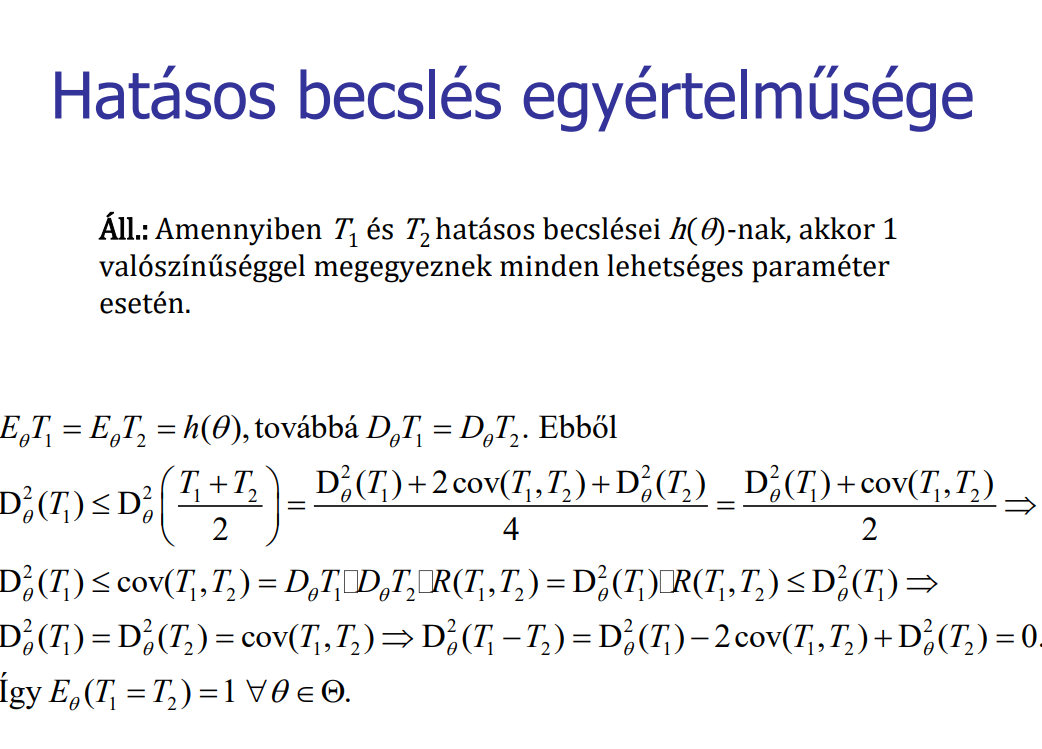
\includegraphics[width=0.7\textwidth]{hatasos_becsles_egyert.png}
        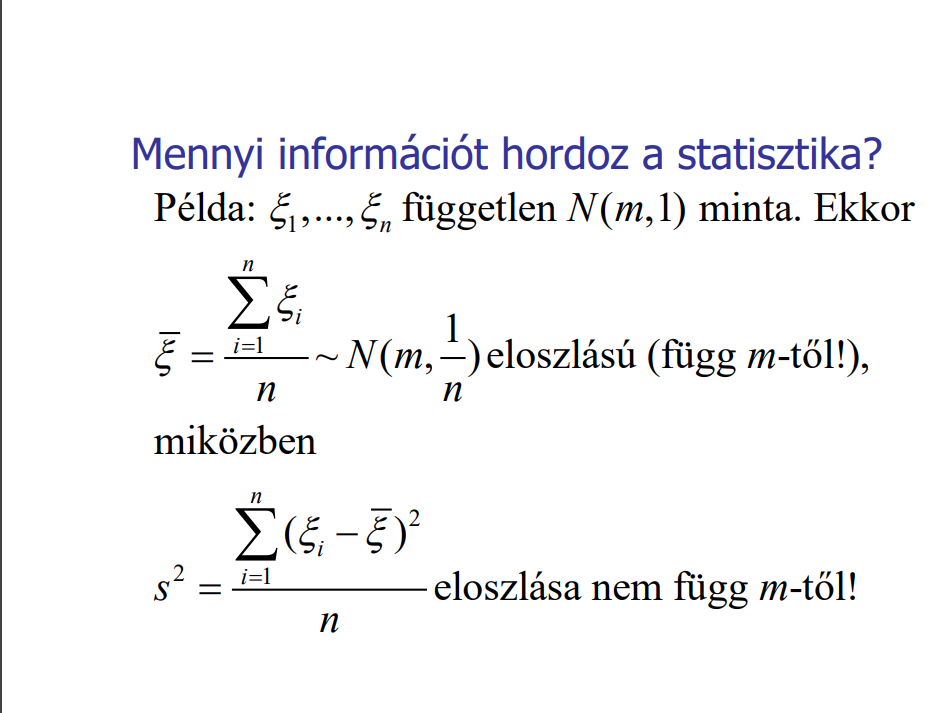
\includegraphics[width=0.7\textwidth]{2.png}
    \end{figure}

    \newpage
    \subsection{Elégséges statisztika}
    \subsection{Elégséges statisztika diszkrét minta esetén}
    \begin{figure}[h]
        \centering
        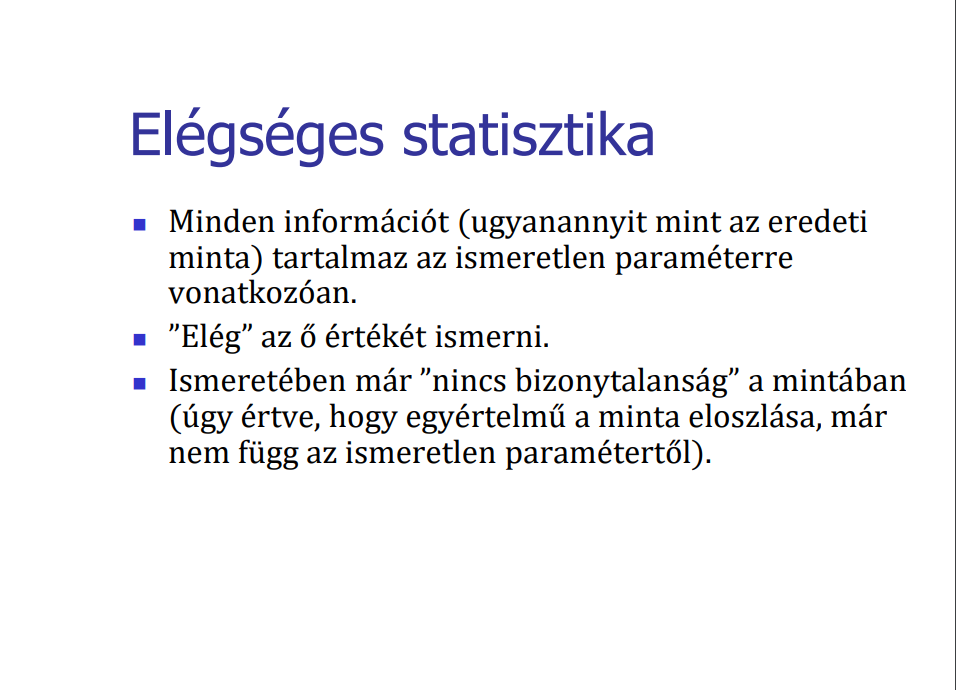
\includegraphics[width=0.7\textwidth]{3.png}
        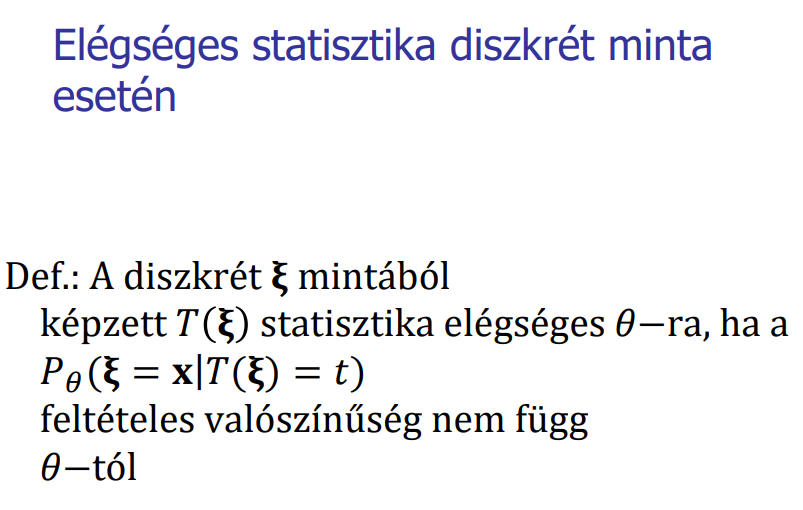
\includegraphics[width=0.7\textwidth]{4.png}
    \end{figure}

    
    \newpage
    \subsection{Feltételes várható érték}
    \subsection{Indikátor példa}
    \begin{figure}[h]
        \centering
        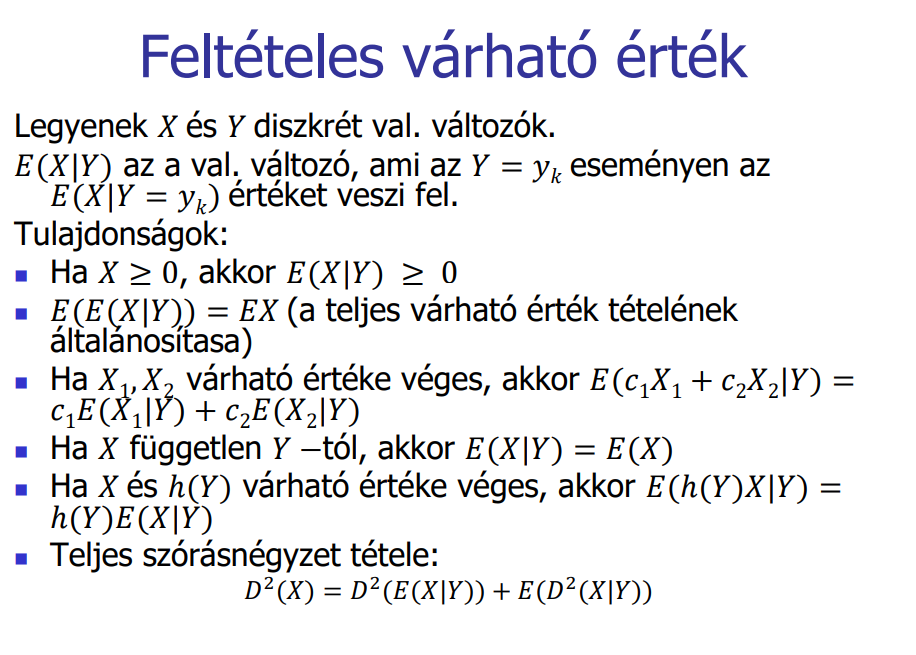
\includegraphics[width=0.7\textwidth]{5.png}
        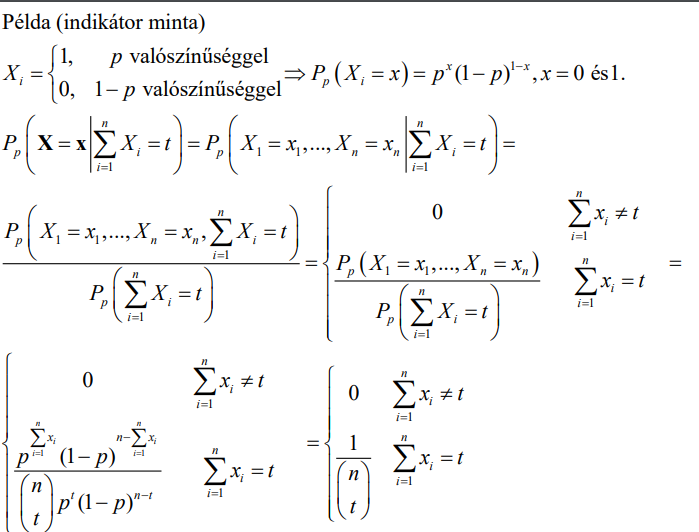
\includegraphics[width=0.7\textwidth]{6.png}
    \end{figure}

    \newpage
    \subsection{Neyman-féle faktorizációs}
    \subsection{Poisson példa}
    \begin{figure}[h]
        \centering
        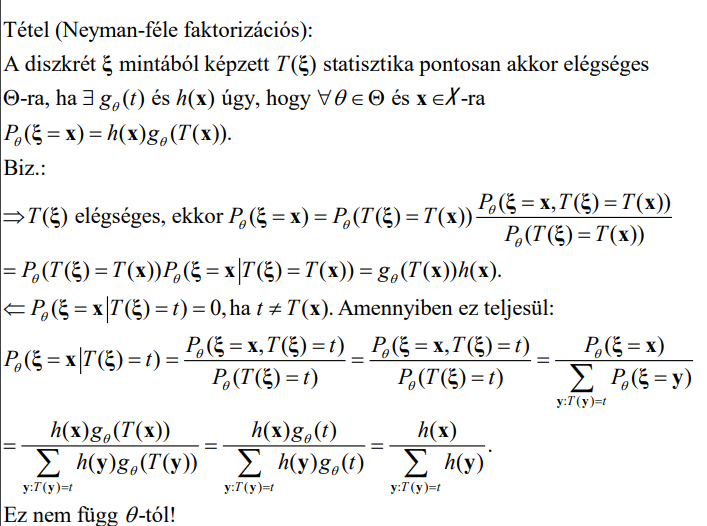
\includegraphics[width=0.7\textwidth]{7.png}
        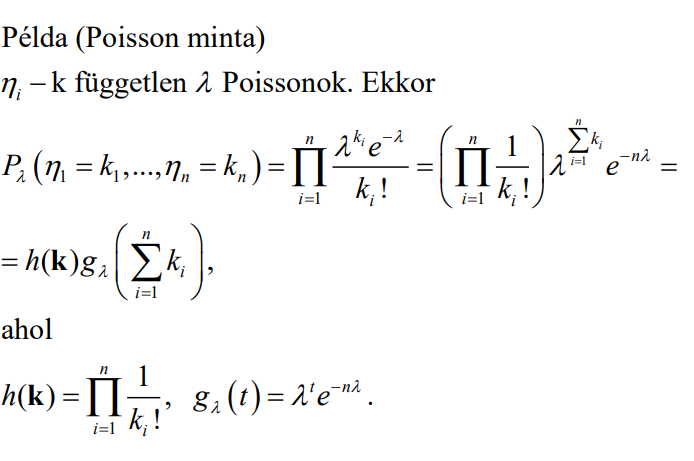
\includegraphics[width=0.7\textwidth]{8.png}
    \end{figure}

    \newpage
    \subsection{Elégséges statisztika általában}
    \subsection{Abszolút folytonos eset}
    \begin{figure}[h]
        \centering
        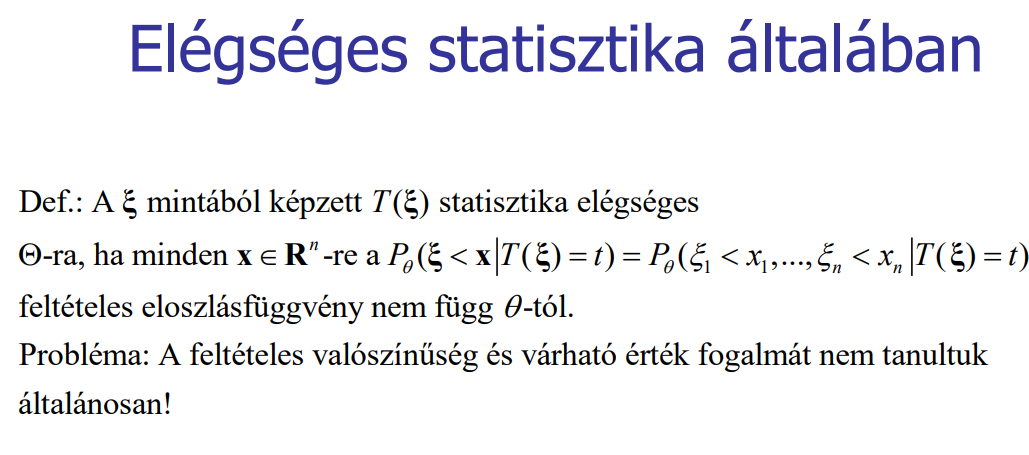
\includegraphics[width=0.7\textwidth]{9.png}
        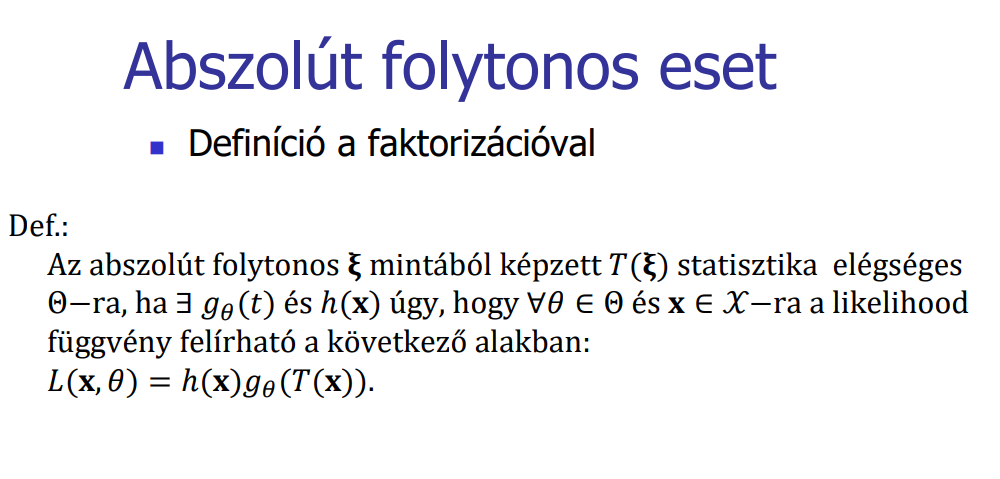
\includegraphics[width=0.7\textwidth]{10.png}
    \end{figure}

    \newpage
    \subsection{Példa normális eloszlásra}
    \subsection{Pédla egyenletes eloszlásra}
    \begin{figure}[h]
        \centering
        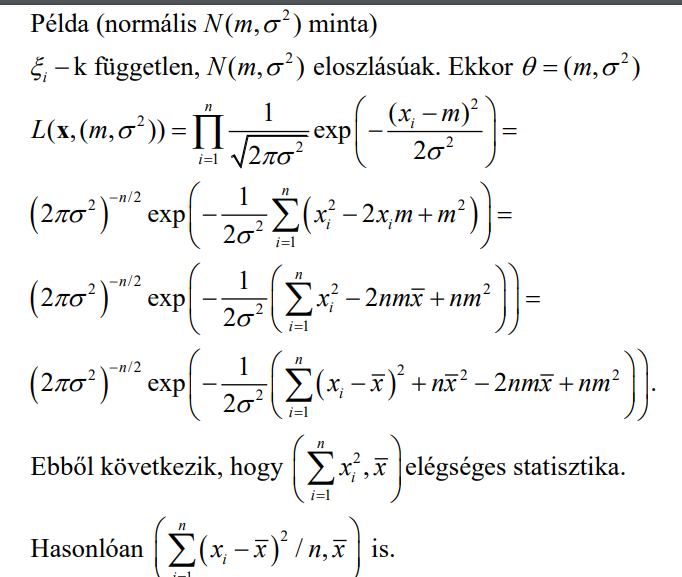
\includegraphics[width=0.7\textwidth]{11.png}
        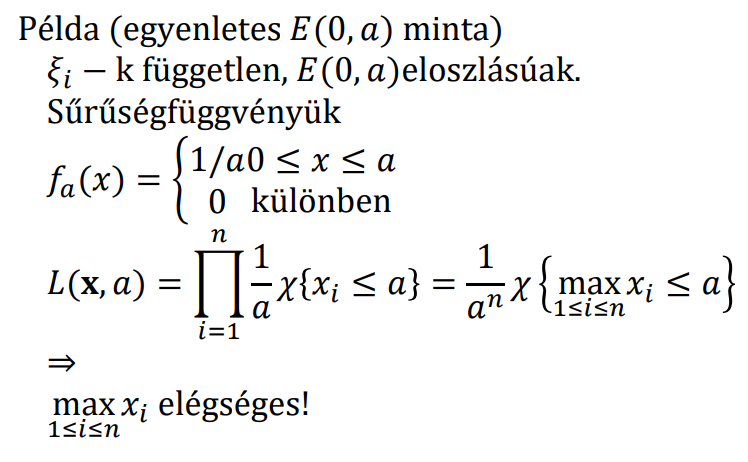
\includegraphics[width=0.7\textwidth]{12.png}
    \end{figure}

    \newpage
    \subsection{Maximum likelihood becslés}
    \subsection{momentum módszer}
    \begin{figure}[h]
        \centering
        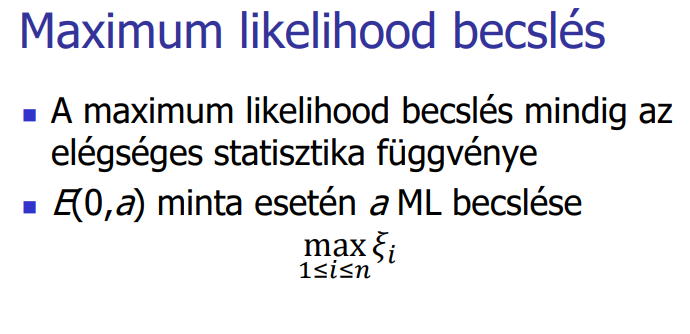
\includegraphics[width=0.7\textwidth]{13.png}
        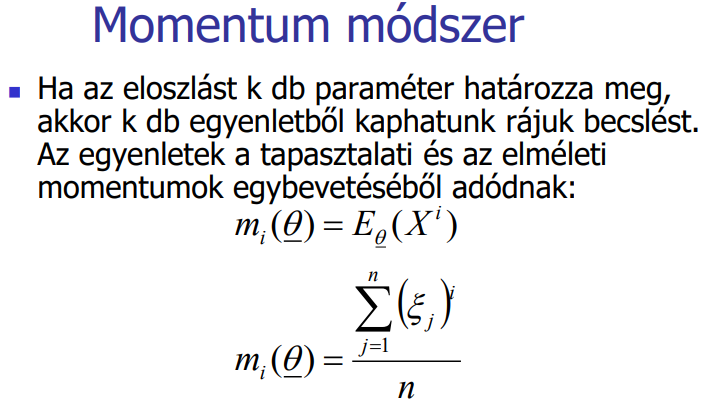
\includegraphics[width=0.7\textwidth]{14.png}
    \end{figure}

\end{document}